\section{Ungesteuerter Gleichrichter M1U}


\begin{tabu}{|l|l|m{0.3\textwidth}}
\cline{1-2}
  Mittelwert
  	& $ \begin{aligned}
  			U_{R AV} &= \frac{1}{T}\int\limits_{0}^{T}u_{R}(t)dt = \frac{1}{2\pi}\int\limits_{0}^{\pi}\hat{U}_{2} \cdot sin(\alpha)d\alpha, \qquad \alpha = \omega t\\
  					&= -\frac{\hat{U}_{2}}{2\pi}(cos(\pi)-cos(0))= \frac{\hat{U}_{2}}{\pi}
  		\end{aligned}$
  	& \multirow{7}{*}[4cm]{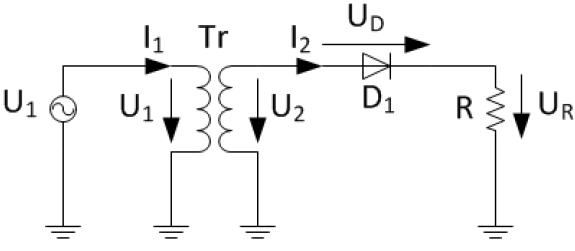
\includegraphics[width = \linewidth]{./pictures/m1u.png}}\\
  	\cline{1-2}
  bei f = 50 Hz 
  	& $U_{R AV} = \frac{1}{20 ms}\int\limits_{0}^{10 ms}u_{R}(t)dt, T = \frac{1}{f}$ &\\
  	\cline{1-2}
  Effektivwert 
  	& $U_{R RMS} = \sqrt{\frac{1}{T}\int\limits_{0}^{T}u_{R}^2 \cdot dt} = \sqrt{\frac{1}{2\pi}\int\limits_{0}^{\pi}\hat{U}_{2}^2 \cdot sin^2(\alpha) \cdot d\alpha} = \frac{\hat{U}_{2}}{2}$ &\\
  	\cline{1-2}
  Allgemein 
  	& $\int\limits_{0}^{\pi}sin^2(\alpha) \cdot d\alpha = \frac{\pi}{2}$&\\
  	\cline{1-2}
  bei f = 50 Hz 
  	& $U_{R RMS} = \sqrt{\frac{1}{20 ms}\int\limits_{0}^{10 ms}u_{R}^2 \cdot dt}$&\\
  	\cline{1-2}
  Laststrom 
  	& $i_{R}(t) = \frac{u_{R}(t)}{R}$&\\
  	\cline{1-2}
  Wirkleistung 
  	& $P = \frac{1}{2\pi}\int\limits_{0}^{\pi}\frac{u_{R}^2(\alpha)}{R} \cdot d\alpha = \frac{U_{R RMS}^2}{R} = \frac{\hat{U}_{2}^2}{4R}$&\\
\cline{1-2}
\end{tabu}
